\chapter{Experimental Study}\label{expstudy}

\section{Introduction}
An experiment is a procedure carried out to support, refute, or validate a hypothesis. Experiments
provide insight into cause-and-effect by demonstrating what outcome occurs when
a particular factor is manipulated. Experiments vary greatly in goal and scale, but always rely
on repeatable procedure and logical analysis of the results. In engineering and the physical
sciences, experiments are a primary component of the scientific method. They are used to
test theories and hypotheses about how physical processes work under particular conditions.
Typically, experiments in these fields focus on replication of identical procedures in hopes of
producing identical results in each replication. No theory can have a real significance without
an experimentation on that theory. To establish some kind of proposition we must have conducted
some experiments and anlysis it’s output results. It is true for our three methods also.
That’s why we have arranged some experiments to test our studied methods.

In this chapter, at first, we have introuduced the data sets on which experiments are conducted.
Then we have discussed about the parameters which are used to determine cluster characteristic.
Then we discussed about different kinds of outcome of the experiments.

\section{Data Sets}
We've used different datasets and applied three methods i.e. \textit{Elbow Method}, \textit{Average Silhouette Method},
\textit{Gap Statistic Method} for finding optimal number of clusters in the dataset. Attribute informations of different datasets are described below:

\begin{enumerate}
\item \textbf{Iris Data Set} : This is perhaps the best known database to be found in the pattern recognition literature.
Fisher's paper is a classic in the field and is referenced frequently to this day. The data set contains 3 classes of 50
instances each, where each class refers to a type of iris plant. One class is linearly separable from the other 2;
the latter are NOT linearly separable from each other. This is an exceedingly simple domain.

\begin{itemize}
\item sepal length in cm
\item sepal width in cm
\item petal length in cm
\item petal width in cm
\item class:
\begin{itemize}
\item Iris Setosa
\item Iris Versicolour
\item Iris Virginica
\end{itemize}
\end{itemize}

\item \textbf{Violent Crime Rates by US State} : This data set contains statistics, in arrests per 100,000 residents for assault, murder,
and rape in each of the 50 US states in 1973. Also given is the percent of the population living in urban areas.
A data frame with 50 observations on 4 variables.
\begin{itemize}
\item	\textit{Murder} -	Numeric	Murder arrests (per 100,000)
\item	\textit{Assault} - Numeric	Assault arrests (per 100,000)
\item	\textit{UrbanPop} -	Numeric	Percent urban population
\item	\textit{Rape} - Numeric	Rape arrests (per 100,000)
\end{itemize}

\item \textbf{Bivariate Data Set} : An artificial data set consisting of 3000 points
in 3 well-separated clusters of size 1000 each. A data frame with 3000 observations on
2 numeric variables giving the x and y coordinates of the points, respectively.

\item \textbf{Isotopic Composition Plutonium Batches} : The pluton data frame has 45 rows and
4 columns, containing percentages of isotopic composition of 45 Plutonium batches.
This data frame contains the following columns:
\begin{itemize}
\item \textit{$Pu_{238}$} - Percentages of the \textit{$Pu_{238}$} isotope, always less than 2 percent.
\item \textit{$Pu_{239}$} - Percentages of the \textit{$Pu_{239}$} isotope, typically between 60 and 80 percent
(from neutron capture of Uranium, \textit{$U_{238}$}).
\item \textit{$Pu_{240}$} Percentage of the \textit{$Pu_{240}$} isotope.
\item \textit{$Pu_{241}$} Percentage of the \textit{$Pu_{241}$} isotope.
\end{itemize}

\item \textbf{Ruspini Data Set} : The Ruspini data set, consisting of 75 points in four groups that
is popular for illustrating clustering techniques. A data frame with 75 observations on 2 variables giving
the x and y coordinates of the points, respectively.

\item \textbf{Wine Data Set} : These data are the results of a chemical analysis of wines grown
in the same region in Italy but derived from three different cultivators. The analysis determined
the quantities of 13 constituents found in each of the three types of wines. All attributes are continuous.

\item \textbf{Votes for Republican Candidate in Presidential Elections} : A data frame with the percents
of votes given to the republican candidate in presidential elections from 1856 to 1976. Rows represent the
50 states, and columns the 31 elections.

\end{enumerate}


\section{Performance Metric}
Different clustering algorithms usually lead to different clusters of data; even for the same
algorithm, the selection of different parameters or the presentation order of data objects
may greatly affect the final clustering partitions. Thus, effective evaluation standards and
criteria are critically important to give users confidence regarding the clustering results. At
the same time, these assessments also provide some meaningful insights on how many clusters
are hidden in the data.

In fact, in most real life clustering situations, the user faces the dilemma of selecting the number
of clusters or partitions in the underlying data. As such, numerous indices for determining
the number of clusters in a data set have been proposed.

All these clustering validity indices combine information about intracluster compactness and
intercluster isolation, as well as other factors, such as geometric or statistical properties of
the data, the number of data objects and dissimilarity or similarity measurements.

\begin{itemize}
\item \textbf{Elbow Index} : The basic\index{Elbow Index} idea behind partitioning methods, such as k-means clustering,
is to define clusters such that the total intra-cluster variation (known as total within-cluster
variation or total within-cluster sum of square) is minimized:\\\\
$minimize(\sum_{k=1}^{K}WC_k)$;

where $C_k$ is the $k^{th}$ cluster and $W(C_k)$ is the within-cluster variation.
That means the total within-cluster sum of square $(wss)$ measures the compactness of the clustering and we want
it to be as small as possible.

\item \textbf{Silhouette index} : Rousseeuw~\cite{rousseeuw87} introduced the silhouette index\index{Silhouette Index} computed using
the following equation:\\\\
Silhouette = $\frac{\sum_{i=1}^{n}S(i)}{n}$; Silhouette $\epsilon{[-1, 1]}$

where,
\begin{itemize}
\item $S(i) = \frac{b(i)−a(i)}{max\{a(i), b(i)\}}$
\item $a(i) = \frac{\sum_{j\epsilon\{C_r, i\}}d_{ij}}{n_r - 1}$ is the average dissimilarity of the ith object
to all other objects of cluster $C_r$
\item $b(i) = \min(d_{iC_{s}})$; $s \neq r$
\item $d_{iC_{s}} = \frac{\sum_{j \epsilon C_{s}}d_{ij}}{n_{s}}$
\end{itemize}

The maximum value of the index is used to determine the optimal number of clusters in the
data~\cite{rousseeuw90}. $S(i)$ is not defined for $k = 1$ (only one cluster).

\item \textbf{Gap Index} : The estimated Gap statistic\index{Gap Index} proposed by Tibshirani~\cite{tibshirani01} is
computed using the following equation:\\

$Gap(q) = \frac{1}{B}\sum_{b=1}^{B} \log{W_{qb}} - \log{W_{q}}$\\

where $B$ is the number of reference data sets generated using uniform prescription and $W_{qb}$
is the within-dispersion matrix. The optimal number of clusters is chosen via finding the smallest
$q$ such that:\\

$Gap(q) \geq Gap(q+1) - s_{q+1}, (q = 1, ..., n-2)$

where,

\begin{itemize}
\item $s_{q} = sd_{q} \sqrt{1+\frac{1}{B}}$
\item $sd_{q}$ is the standard deviation of $\log{W_{qb}}, b = (1,...,B)$ : $sd_{q} = \sqrt{\frac{1}{B}\sum_{b=1}^{B}(\log{W_{qb}}-\bar{l})^2}$
\item $\bar{l} = \frac{1}{B}\sum_{b=1}^{B}(\log{W_{qb}}) $
\end{itemize}

\end{itemize}

\section{Results}
We have applied three different methods i.e. elbow method, silhoutte method and gap statistic method on
various datasets and output the optimal number of clusters the method suggests. Now we will see the outputs
generated for three methods in the following section:

\begin{itemize}
\item \textbf{Elbow Method} : Here we plot Total within sum of square (wss)\index{WSS} along the Y-axis and
Number of clusters $K$ along the X-axis. The total within-cluster sum of square (wss) measures the compactness
of the clustering and we want it to be as small as possible. And from the algorithm we know that The location
of a bend (knee) in the plot is generally considered as an indicator of the appropriate number of clusters.

In Figure \ref{fig:elbow1} we can see that three clusters have been suggested for \textit{iris} dataset which
has originally three classes.

\begin{figure}[h!]
  \centering
  \includegraphics[scale=1.3]{figures/results/iris/elbow.png}
  \caption{Elbow Method on Iris Dataset}
  \label{fig:elbow1}
\end{figure}

\vspace{15mm}

In Figure \ref{fig:elbow2} we can see that three clusters have been suggested for \textit{Isotopic Composition Plutonium Batches}
dataset.

\begin{figure}[h!]
  \centering
  \includegraphics[scale=1.3]{figures/results/pluton/elbow.png}
  \caption{Elbow Method on Isotopic Composition Plutonium Batches}
  \label{fig:elbow2}
\end{figure}

\newpage

In Figure \ref{fig:elbow3} we can see that four clusters have been suggested for \textit{Votes for Republican Candidate in Presidential Elections}
dataset.

\begin{figure}[h!]
  \centering
  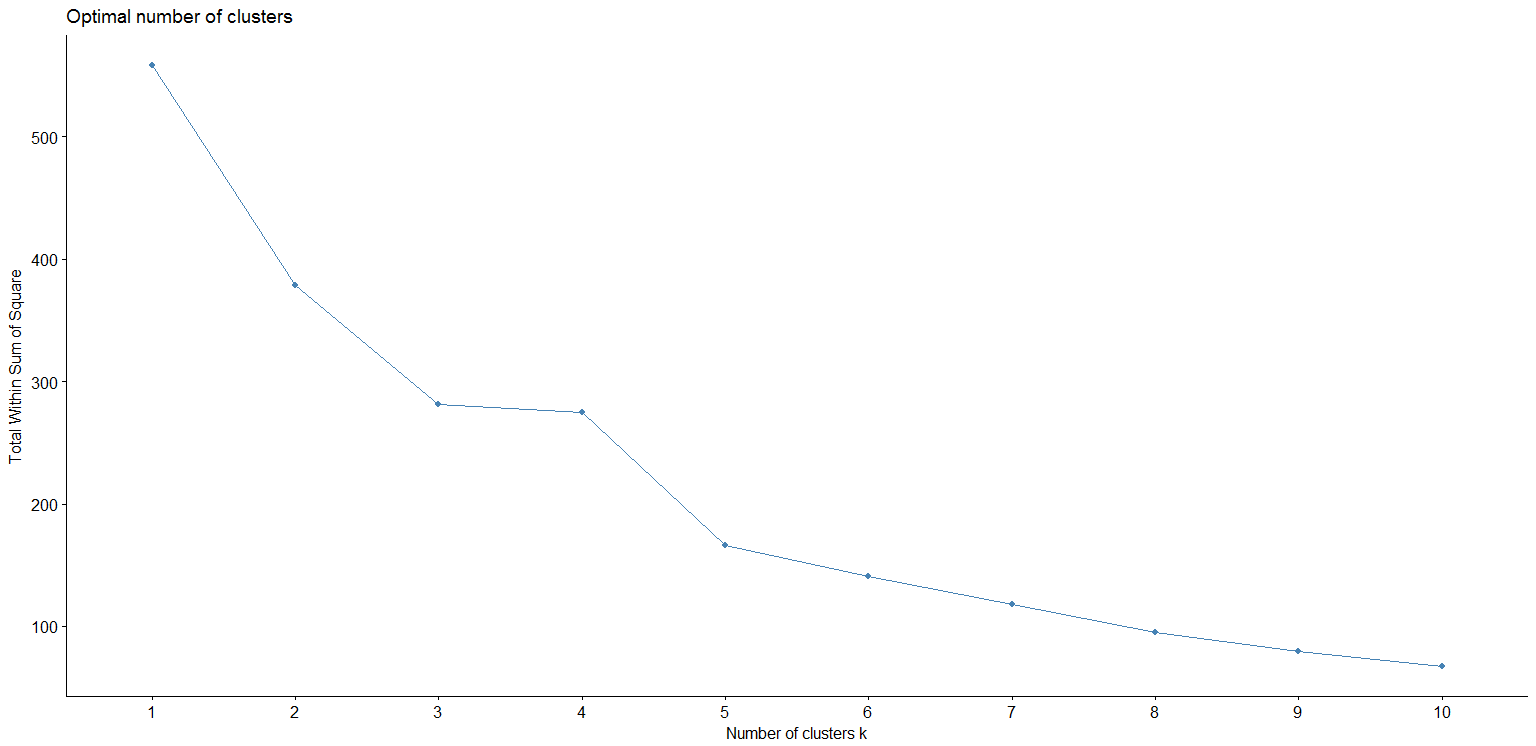
\includegraphics[scale=1.3]{figures/results/republican/elbow.png}
  \caption{Elbow Method on Votes for Republican Candidate in Presidential Elections}
  \label{fig:elbow3}
\end{figure}

\vspace{15mm}

In Figure \ref{fig:elbow4} we can see that four clusters have been suggested for \textit{Ruspini} dataset.

\begin{figure}[h!]
  \centering
  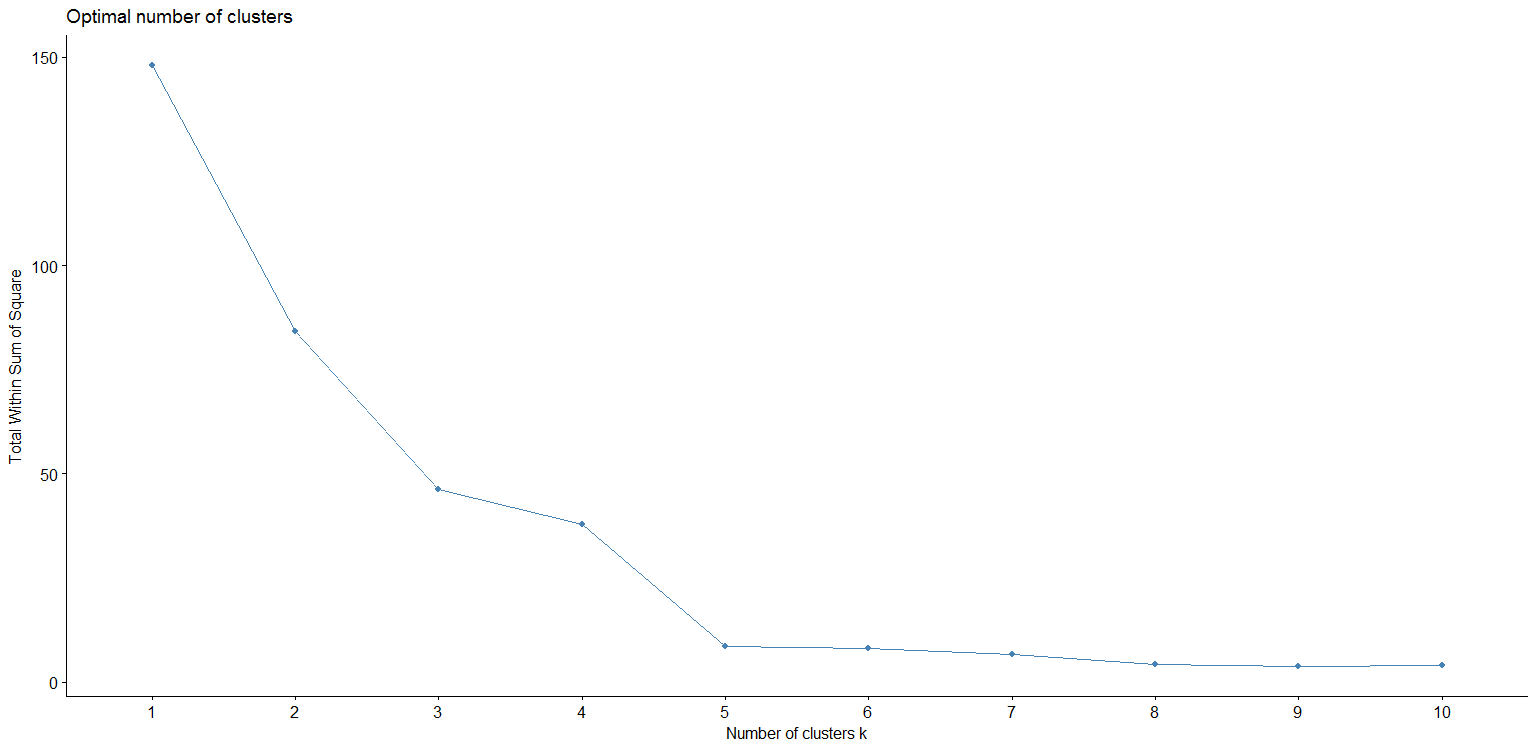
\includegraphics[scale=1.3]{figures/results/ruspini/elbow.png}
  \caption{Elbow Method on Ruspini Dataset}
  \label{fig:elbow4}
\end{figure}

\newpage

In Figure \ref{fig:elbow5} we can see that four clusters have been suggested for \textit{Violent Crime Rates by US State}
dataset.

\begin{figure}[h!]
  \centering
  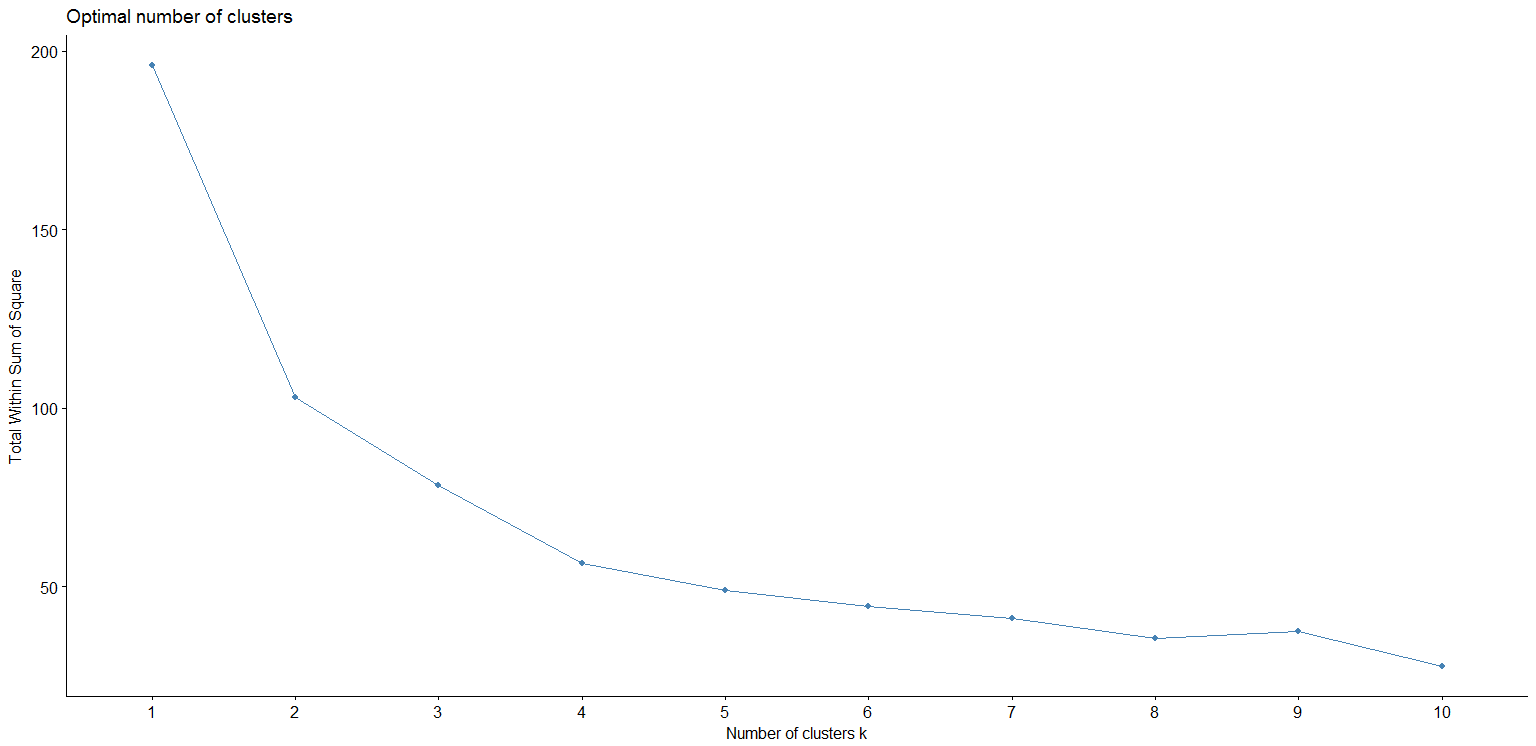
\includegraphics[scale=1.3]{figures/results/USArrests/elbow.png}
  \caption{Elbow Method on Violent Crime Rates by US State}
  \label{fig:elbow5}
\end{figure}

\vspace{15mm}

In Figure \ref{fig:elbow6} we can see that three clusters have been suggested for \textit{Wine} dataset.

\begin{figure}[h!]
  \centering
  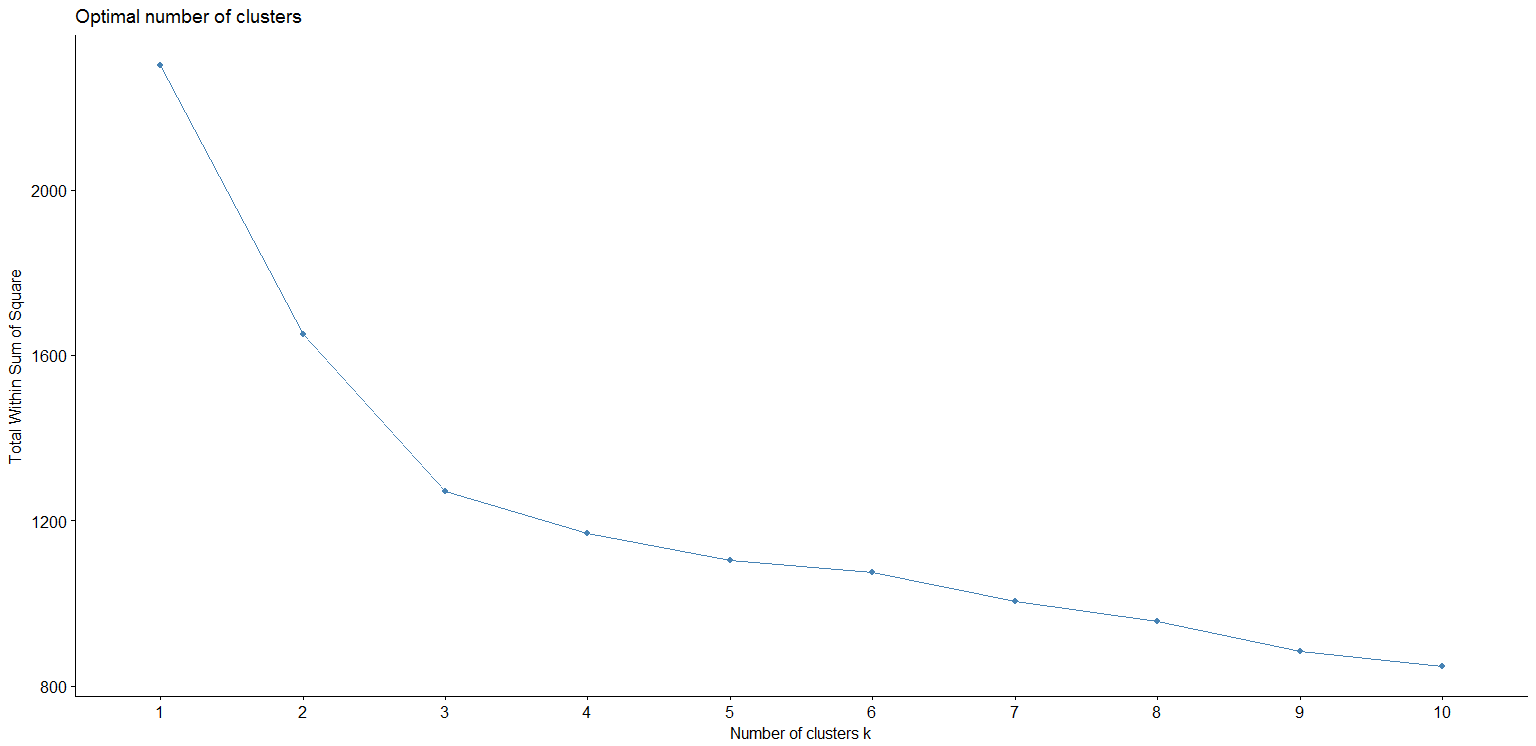
\includegraphics[scale=1.3]{figures/results/wine/elbow.png}
  \caption{Elbow Method on Wine Data Set}
  \label{fig:elbow6}
\end{figure}

\newpage

In Figure \ref{fig:elbow7} we can see that three clusters have been suggested for \textit{Bivariate} dataset.

\begin{figure}[h!]
  \centering
  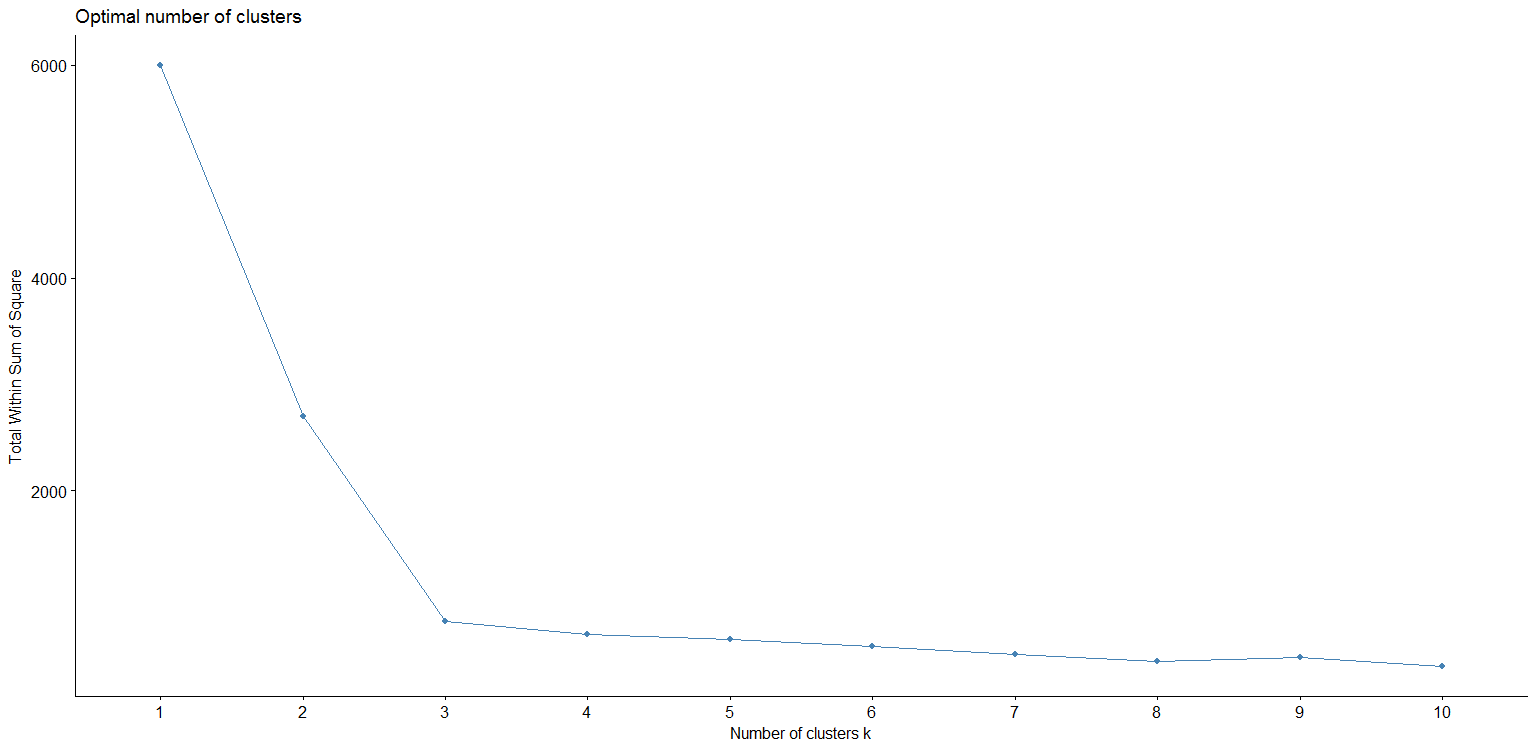
\includegraphics[scale=1.3]{figures/results/xclara/elbow.png}
  \caption{Elbow Method on Bivariate Data Set}
  \label{fig:elbow7}
\end{figure}

\item \textbf{Average Silhoutte Method} : Average silhouette method computes the average silhouette of observations
for different values of $K$. The optimal number of clusters $K$ is the one that maximize the average silhouette over
a range of possible values for $K$. For each $K$, we calculate the average silhouette of all observations (avg.sil)
and the we plot the curve of $avg.sil$ according to the number of clusters $K$. Finally, the location of the maximum
is considered as the appropriate number of clusters.

In Figure \ref{fig:silhoutte1} we can see that two clusters have been suggested for \textit{Iris} Data Set.

\begin{figure}[h!]
  \centering
  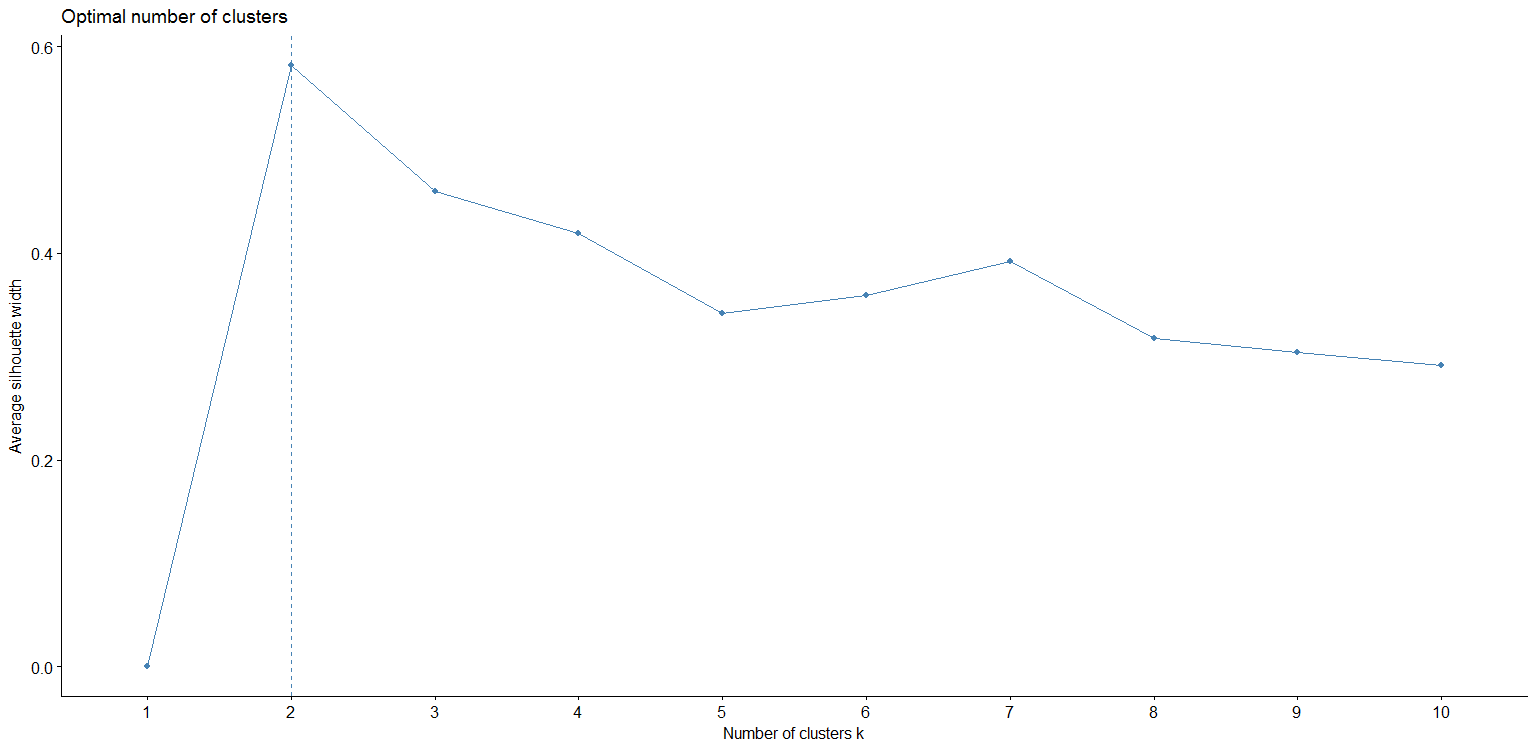
\includegraphics[scale=1.2]{figures/results/iris/silhouette.png}
  \caption{Average Silhouette Method on Iris Dataset}
  \label{fig:silhoutte1}
\end{figure}

In Figure \ref{fig:silhoutte2} we can see that three clusters have been suggested for \textit{Isotopic Composition Plutonium Batches} Data Set.

\begin{figure}[h!]
  \centering
  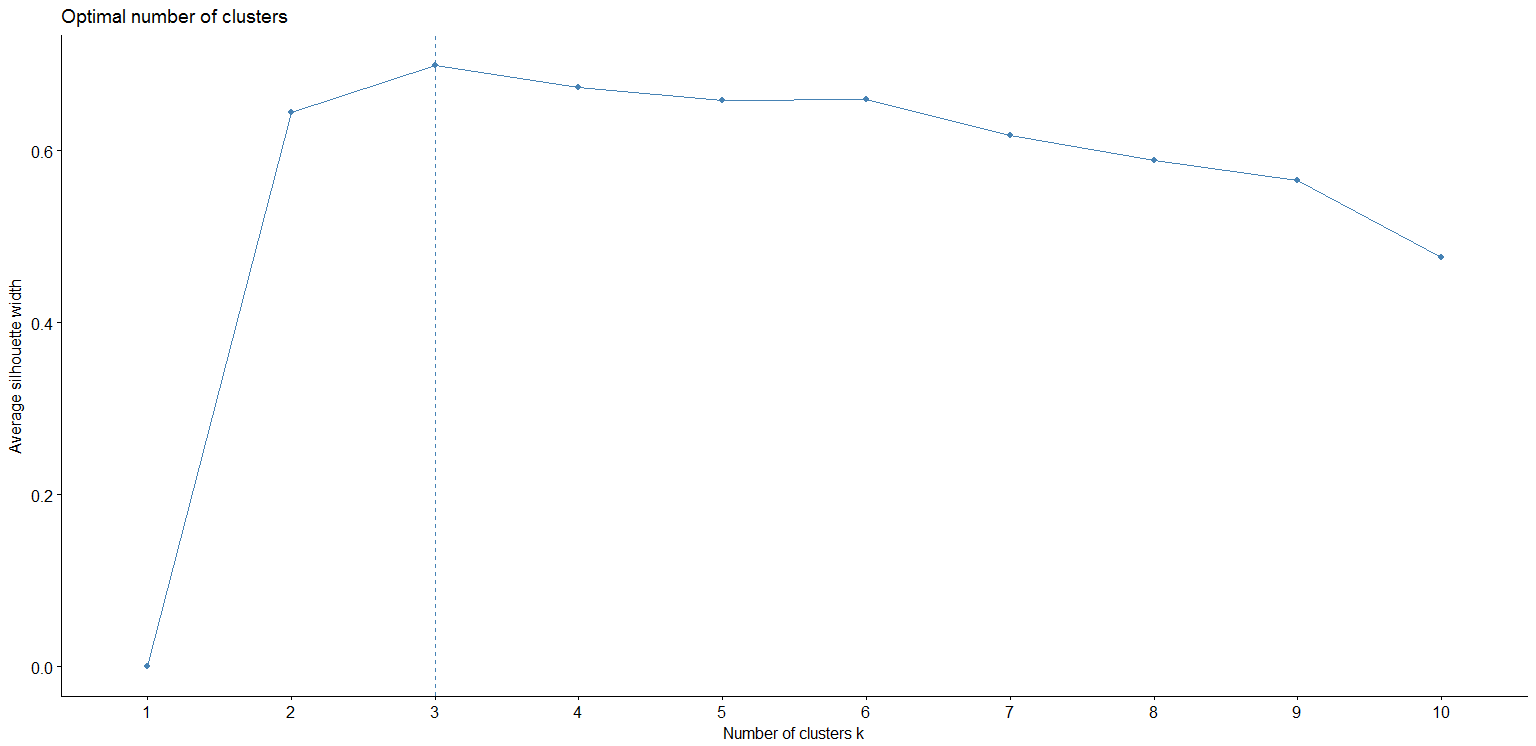
\includegraphics[scale=1.3]{figures/results/pluton/silhouette.png}
  \caption{Average Silhouette Method on Isotopic Composition Plutonium Batches}
  \label{fig:silhoutte2}
\end{figure}

\vspace{15mm}

In Figure \ref{fig:silhoutte3} we can see that four clusters have been suggested for \textit{Votes for Republican Candidate in Presidential Elections} Data Set.

\begin{figure}[h!]
  \centering
  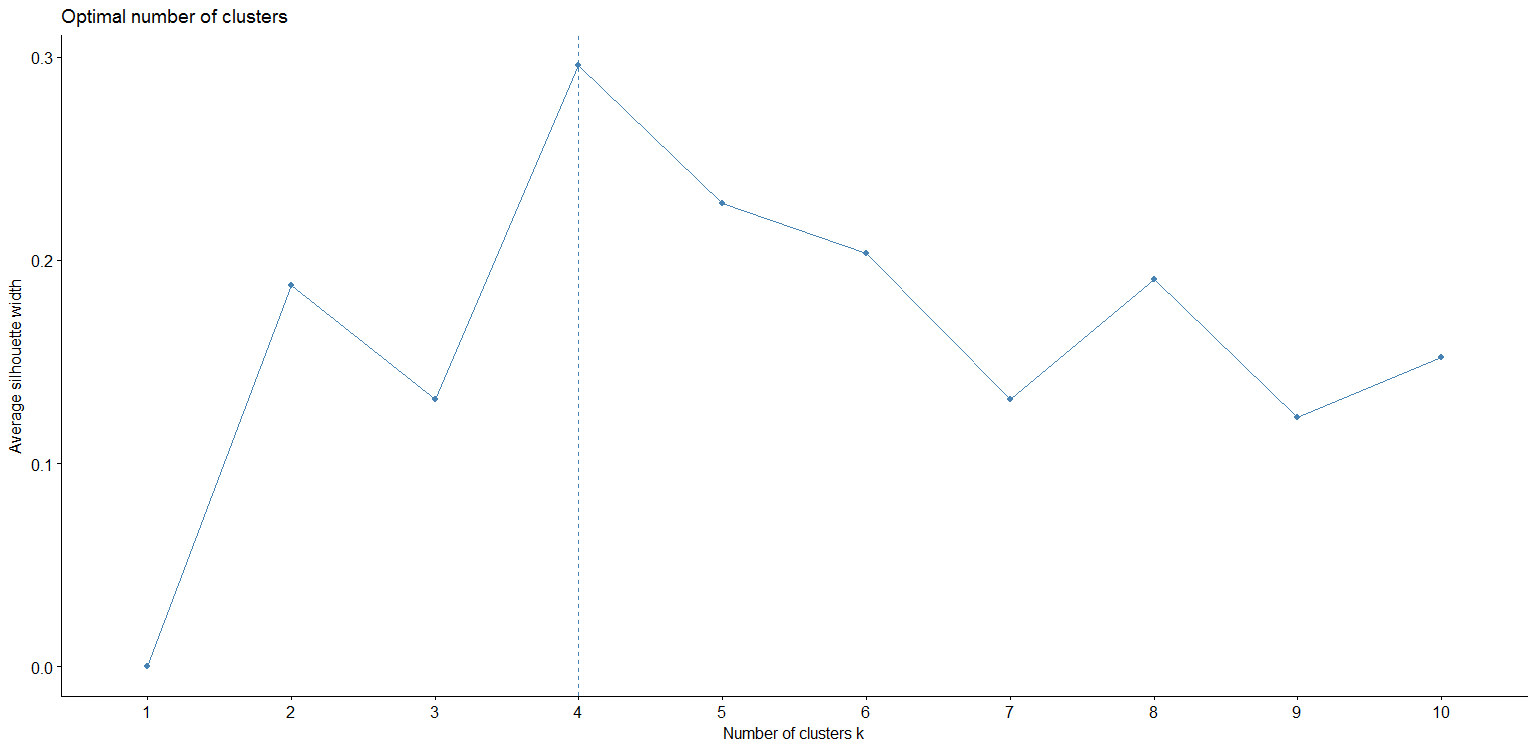
\includegraphics[scale=1.3]{figures/results/republican/silhouette.png}
  \caption{Average Silhouette Method on Votes for Republican Candidate in Presidential Elections}
  \label{fig:silhoutte3}
\end{figure}

\newpage

In Figure \ref{fig:silhoutte4} we can see that six clusters have been suggested for \textit{Ruspini} Data Set.

\begin{figure}[h!]
  \centering
  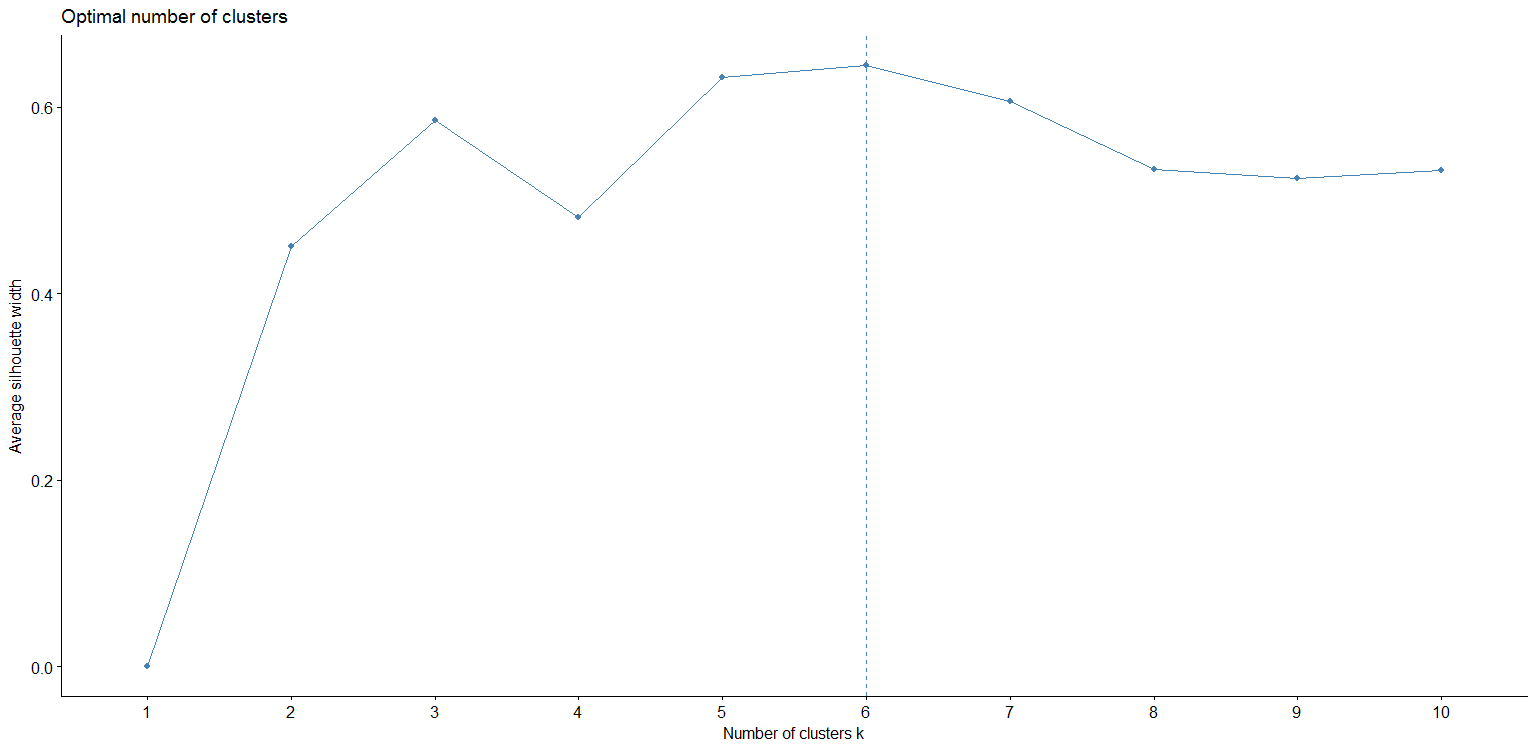
\includegraphics[scale=1.3]{figures/results/ruspini/silhouette.png}
  \caption{Average Silhouette Method on Ruspini Data Set}
  \label{fig:silhoutte4}
\end{figure}

\vspace{15mm}

In Figure \ref{fig:silhoutte5} we can see that two clusters have been suggested for \textit{Violent Crime Rates by US State} Data Set.

\begin{figure}[h!]
  \centering
  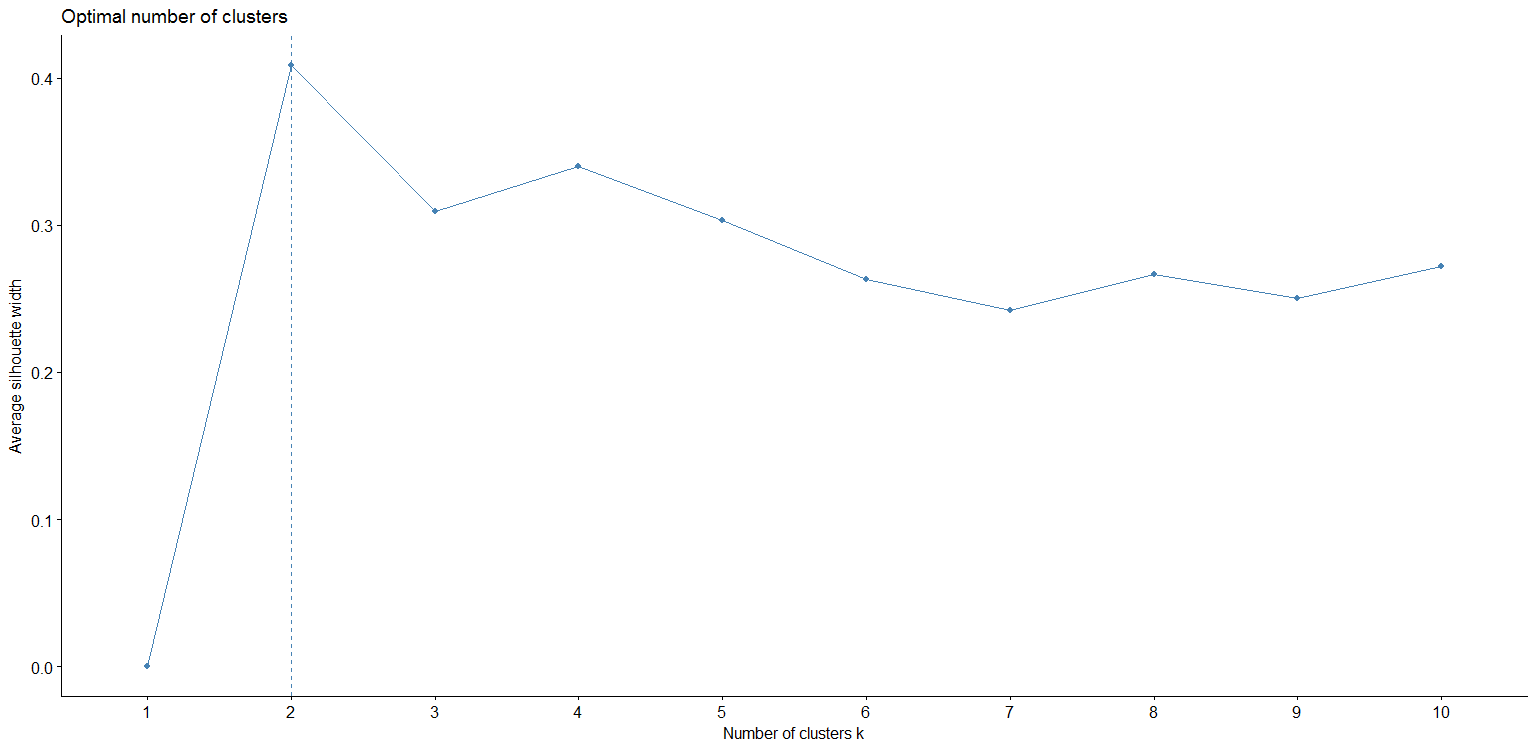
\includegraphics[scale=1.3]{figures/results/USArrests/silhouette.png}
  \caption{Average Silhouette Method on Violent Crime Rates by US State}
  \label{fig:silhoutte5}
\end{figure}

\newpage

In Figure \ref{fig:silhoutte6} we can see that three clusters have been suggested for \textit{Wine} Data Set.

\begin{figure}[h!]
  \centering
  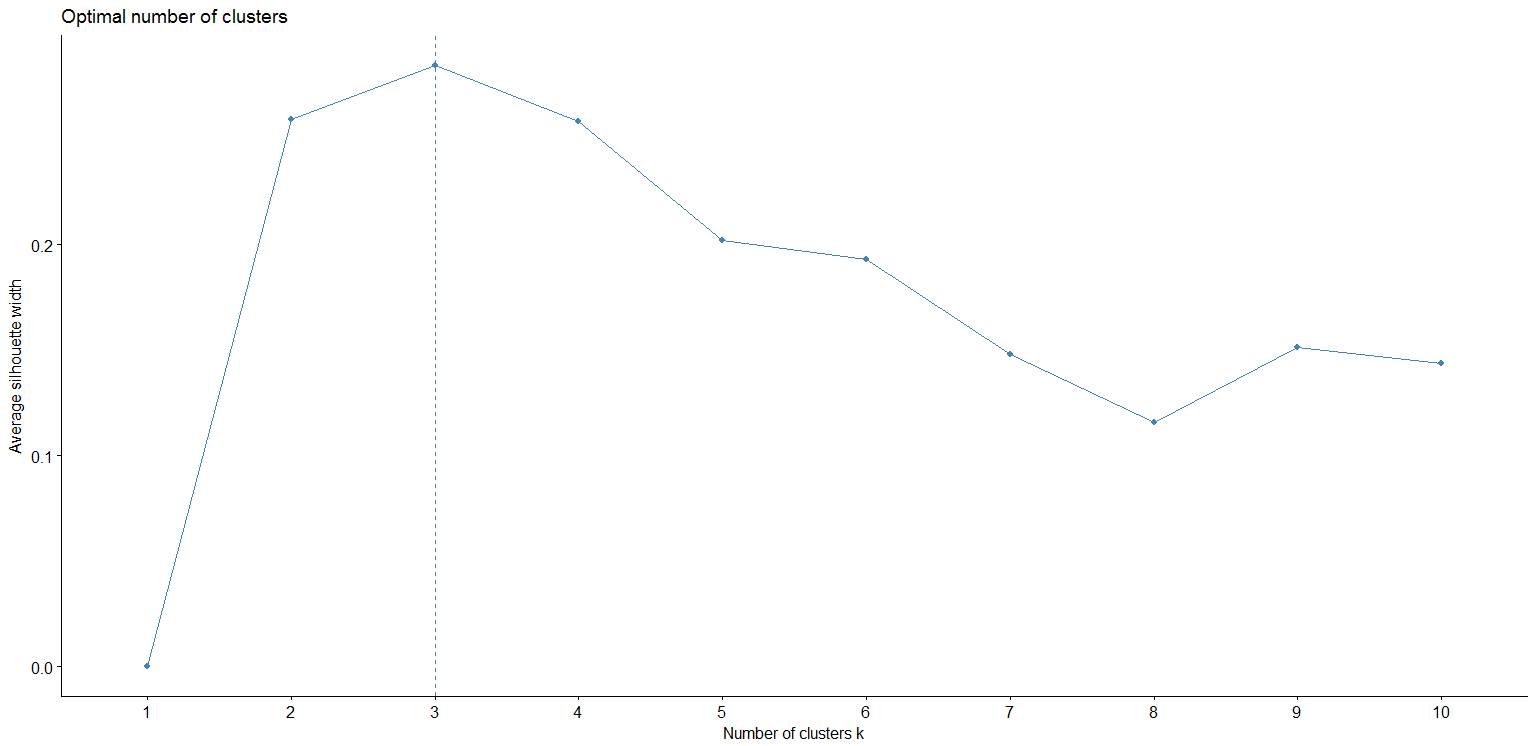
\includegraphics[scale=1.3]{figures/results/wine/silhouette.png}
  \caption{Average Silhouette Method on Wine Data Set}
  \label{fig:silhoutte6}
\end{figure}

\vspace{15mm}

In Figure \ref{fig:silhoutte7} we can see that three clusters have been suggested for \textit{Bivariate} Data Set.

\begin{figure}[h!]
  \centering
  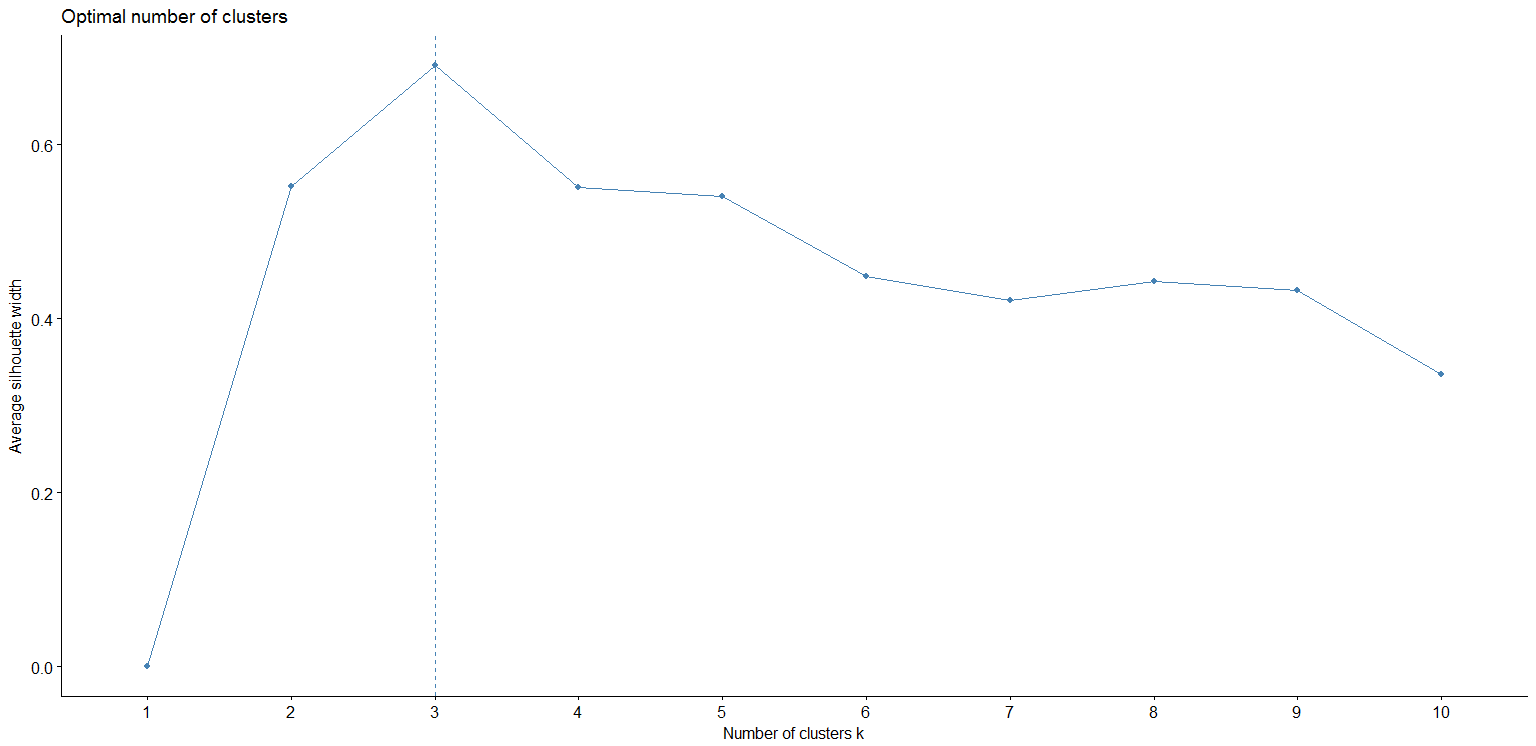
\includegraphics[scale=1.3]{figures/results/xclara/silhouette.png}
  \caption{Average Silhouette Method on Bivariate Data Set}
  \label{fig:silhoutte7}
\end{figure}

\newpage

\item \textbf{Gap Statistic Method} : The gap statistic compares the total within intracluster variation for different
values of $k$ with their expected values under null reference distribution of the data, i.e. a distribution with no
obvious clustering. The reference dataset is generated using \textit{Monte Carlo} Simulations of the sampling process.
That is, for each variable $(x_i)$ in the data set we compute its range $[min(x_i),max(x_j)]$ and generate values
for the $n$ points uniformly from the interval $min$ to $max$. For the observed data and the the reference data, the total
intracluster variation is computed using different values of $k$. The gap statistic for a given $k$ is defined as follow:

$Gap_n(k) = E_n^{*}\{\log W_k\} - \log W_k$

\vspace{15mm}

In Figure \ref{fig:gap1} we can see that three clusters have been suggested for \textit{Iris} Data Set.

\begin{figure}[h!]
  \centering
  \includegraphics[scale=1.3]{figures/results/iris/gap.png}
  \caption{Gap Statistic Method on Iris Dataset}
  \label{fig:gap1}
\end{figure}

\newpage

In Figure \ref{fig:gap2} we can see that seven clusters have been suggested for \textit{Isotopic Composition Plutonium Batches} Data Set.

\begin{figure}[h!]
  \centering
  \includegraphics[scale=1.3]{figures/results/pluton/gap.png}
  \caption{Gap Statistic Method on Isotopic Composition Plutonium Batches}
  \label{fig:gap2}
\end{figure}

\vspace{15mm}

In Figure \ref{fig:gap3} we can see that one cluster have been suggested for \textit{Republican Candidate in Presidential Elections} Data Set.

\begin{figure}[h!]
  \centering
  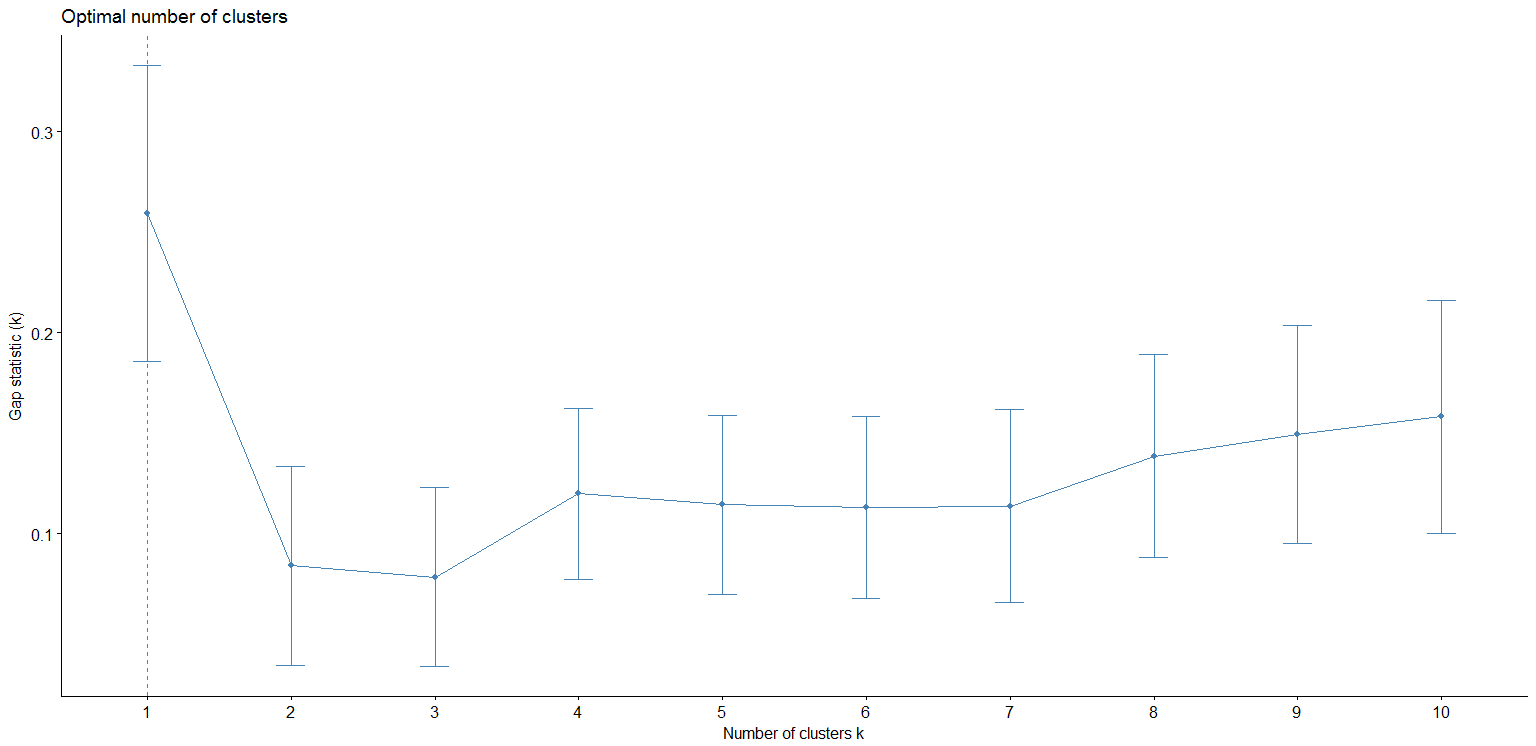
\includegraphics[scale=1.3]{figures/results/republican/gap.png}
  \caption{Gap Statistic Method on Republican Candidate in Presidential Elections}
  \label{fig:gap3}
\end{figure}

\newpage

In Figure \ref{fig:gap4} we can see that four clusters have been suggested for \textit{Ruspini} Data Set.

\begin{figure}[h!]
  \centering
  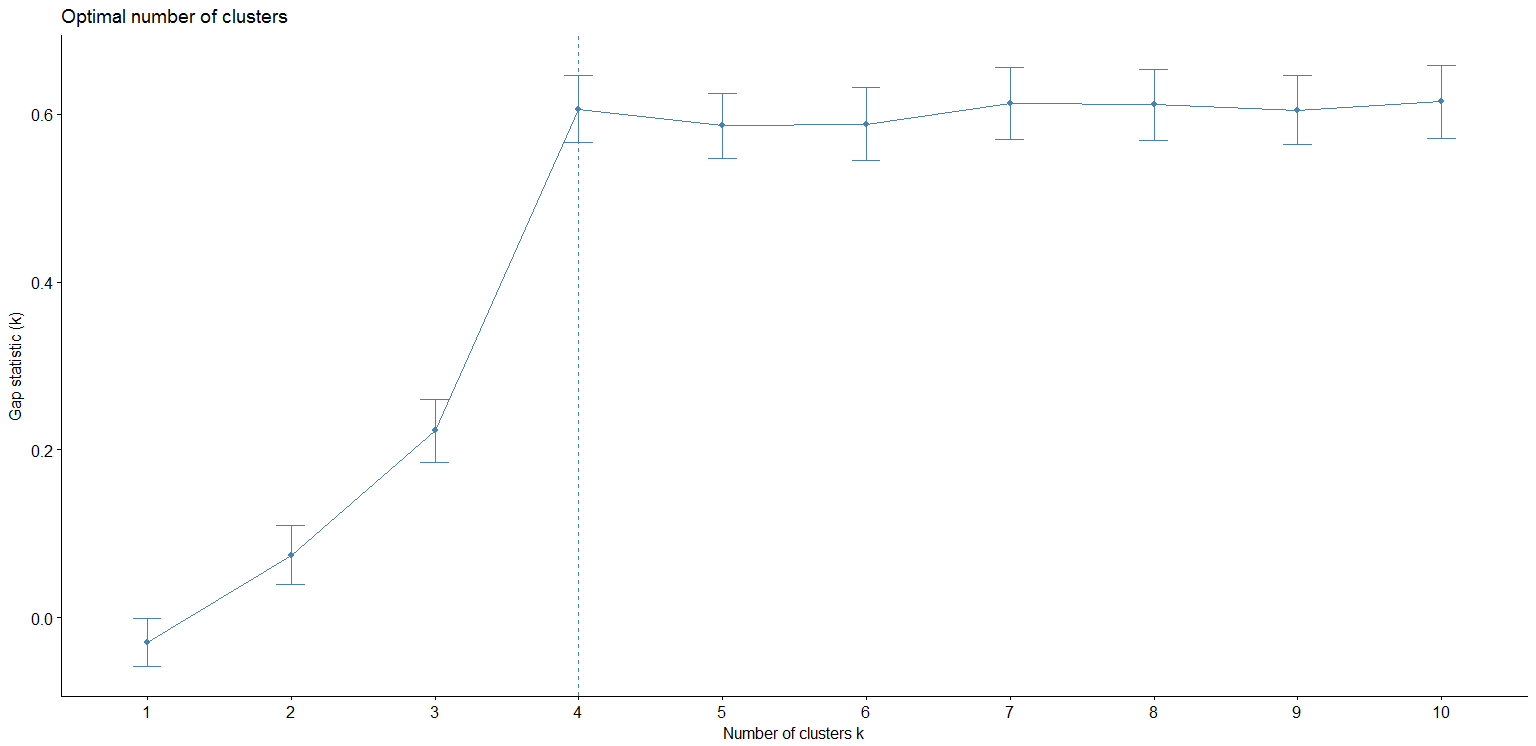
\includegraphics[scale=1.3]{figures/results/ruspini/gap.png}
  \caption{Gap Statistic Method on Ruspini}
  \label{fig:gap4}
\end{figure}

\vspace{15mm}

In Figure \ref{fig:gap5} we can see that four clusters have been suggested for \textit{Violent Crime Rates by US State} Data Set.

\begin{figure}[h!]
  \centering
  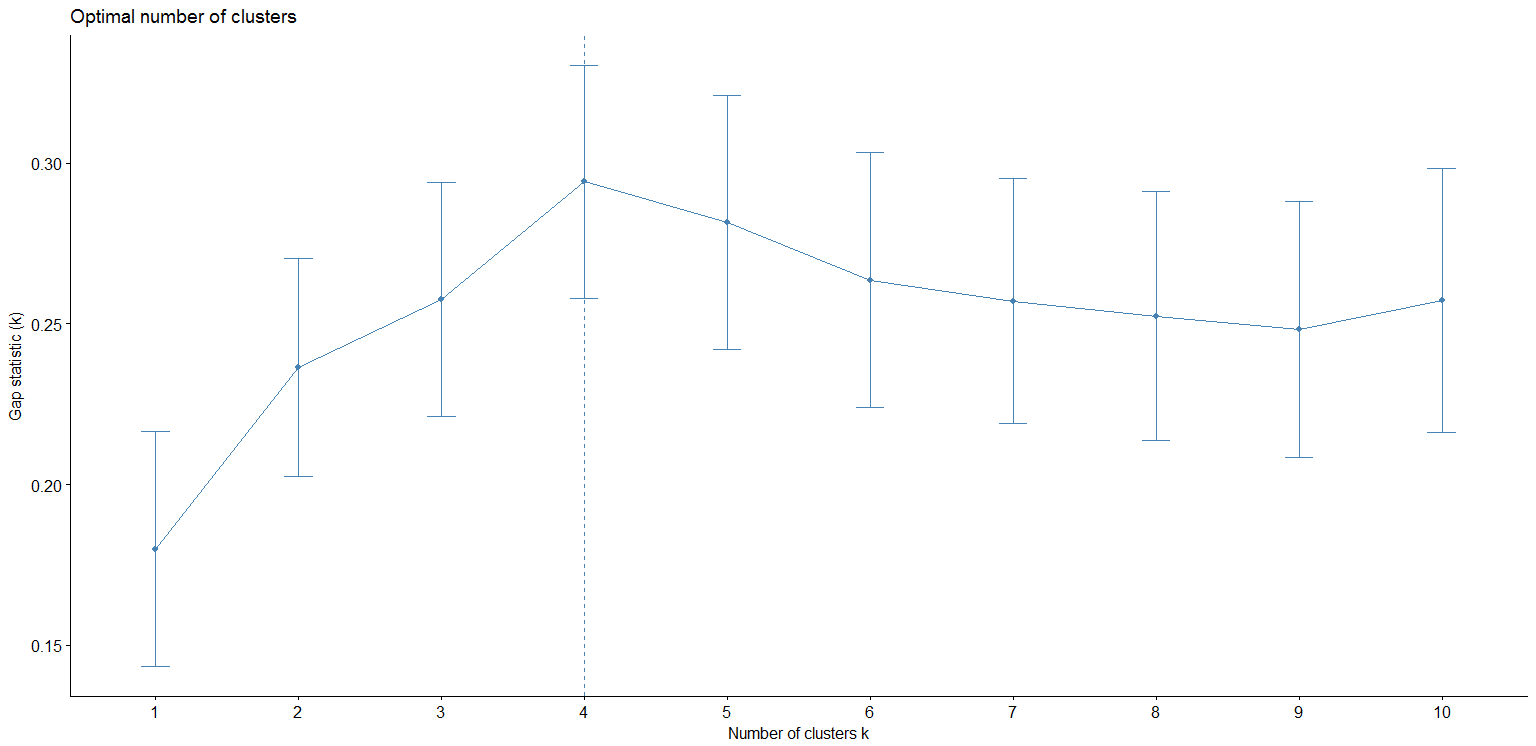
\includegraphics[scale=1.3]{figures/results/USArrests/gap.png}
  \caption{Gap Statistic Method on Violent Crime Rates by US State}
  \label{fig:gap5}
\end{figure}

\newpage

In Figure \ref{fig:gap6} we can see that three clusters have been suggested for \textit{Wine} Data Set.

\begin{figure}[h!]
  \centering
  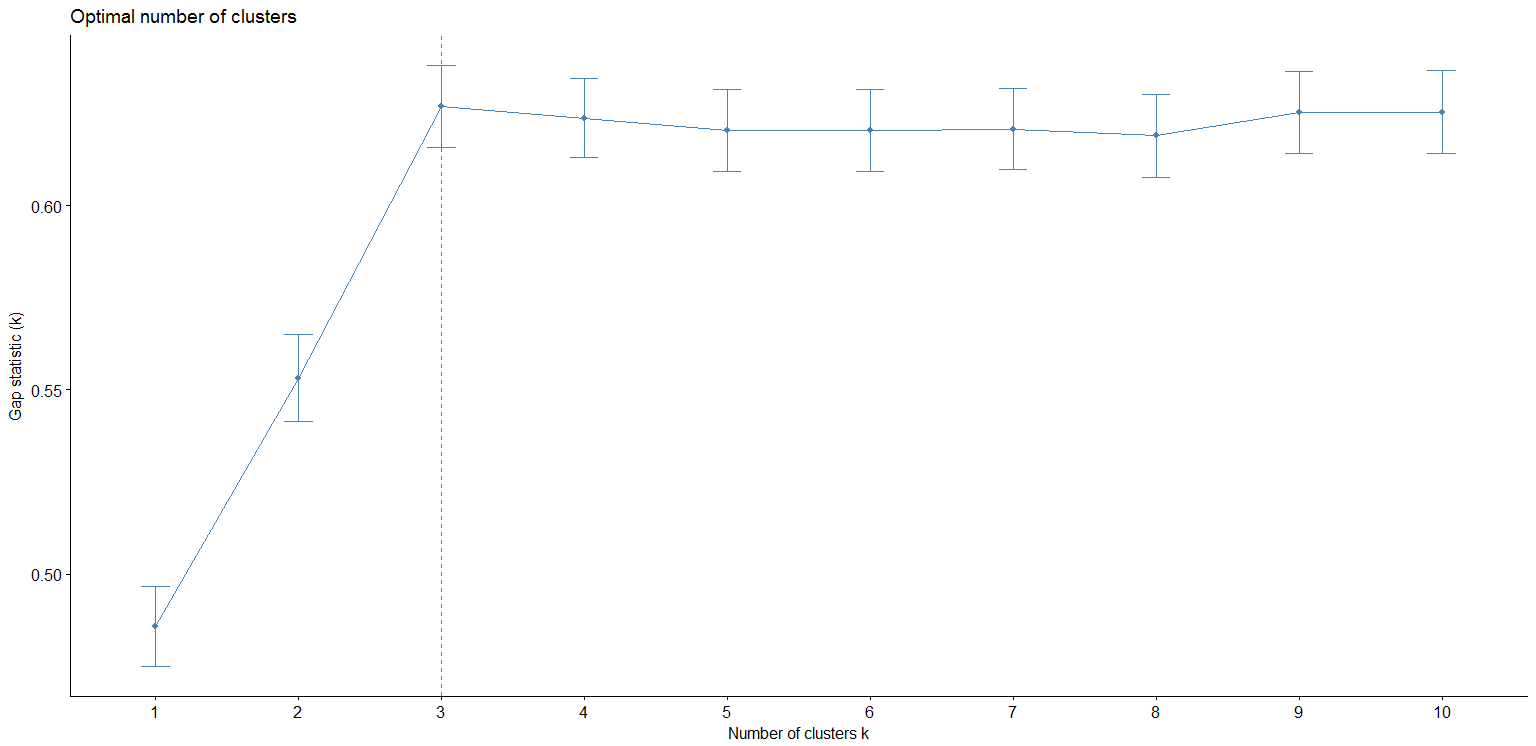
\includegraphics[scale=1.3]{figures/results/wine/gap.png}
  \caption{Gap Statistic Method on Wine Data Set}
  \label{fig:gap6}
\end{figure}

\vspace{15mm}

In Figure \ref{fig:gap7} we can see that three clusters have been suggested for \textit{Bivariate} Data Set.

\begin{figure}[h!]
  \centering
  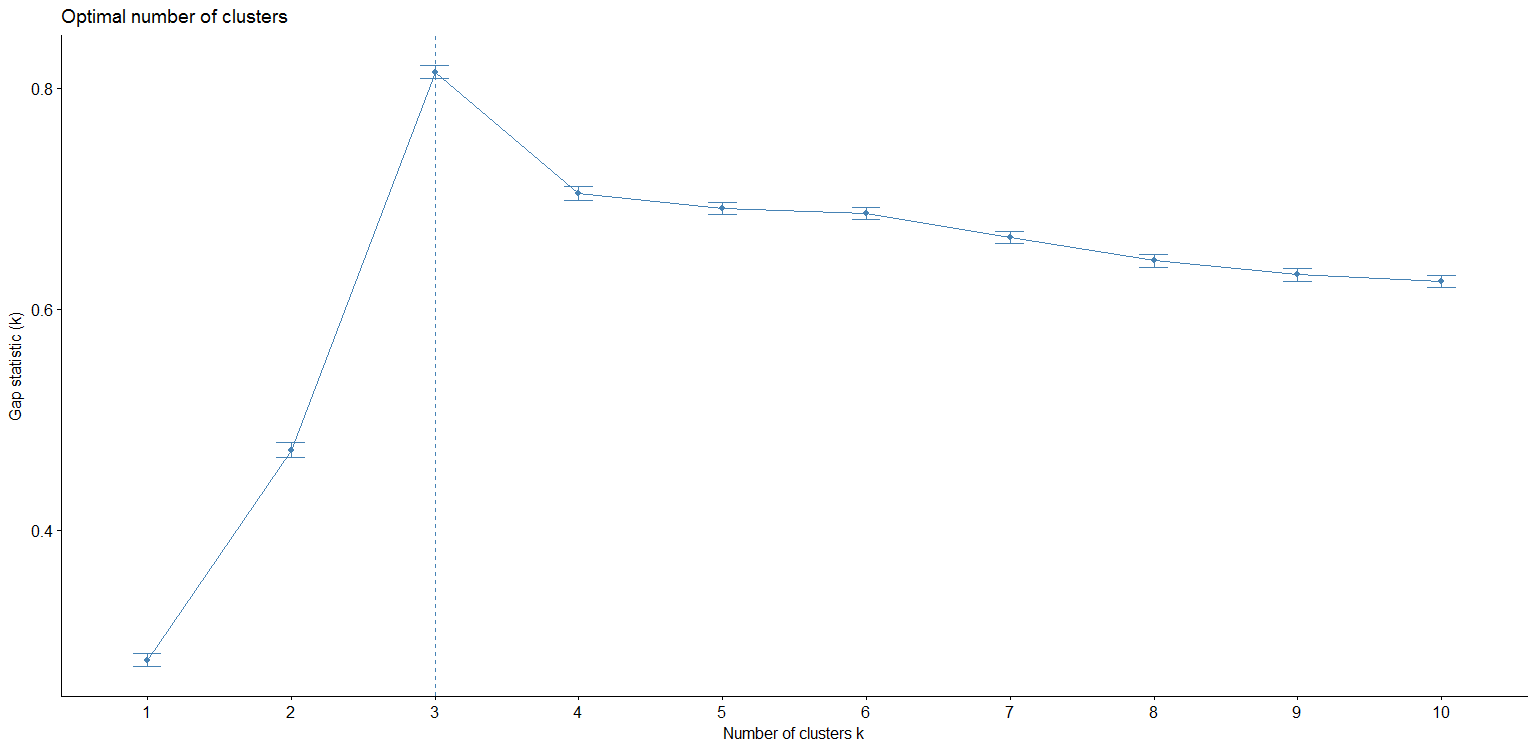
\includegraphics[scale=1.3]{figures/results/xclara/gap.png}
  \caption{Gap Statistic Method on Bivariate Data Set}
  \label{fig:gap7}
\end{figure}

\end{itemize}

\newpage

Now we can make a comparison table to see how different methods are working on different datasets. In Table~\ref{table:1}
we can see original cluster number and output of three methods accordingly.

\begin{table}[h]
 \caption{Table to compare outputs of different methods}
 \begin{tabular}{|C{8.1cm}|C{1.5cm}|C{1.3cm}|C{1.8cm}|C{1.4cm}|}
 \hline
  Data Set & Original Clusters & Elbow Method & Average Silhouette Method & Gap Statistic Method \\ [0.5ex]
 \hline
 \textit{Iris Data Set} & 3 & 3 & 2 & 3 \\
 \hline
 \textit{Bivariate Data Set} & 3 & 3 & 3 & 3 \\
 \hline
 \textit{Violent Crime Rates by US State} & 4 & 4 & 2 & 4 \\
 \hline
 \textit{Ruspini Data Set} & 4 & 4 & 6 & 4 \\
 \hline
 \textit{Isotopic Composition Plutonium Batches} & 3 & 3 & 3 & 7 \\
 \hline
 \textit{Republican Candidate in Presidential Elections} & 4 & 4 & 4 & 1 \\
 \hline
 \textit{Wine Data Set} & 3 & 3 & 3 & 3 \\
 \hline
\end{tabular}
\label{table:1}
\end{table}


\section{Discussion}
The problem of estimating the number of clusters in a data set is difficult, underlined by the
fact that there is no clear definition of a `cluster'. Hence, in data that are not clearly separated
into groups, different people might have different opinions about the number of distinct
clusters. In this paper, we have focused on well-separated clusters and have proposed the
gap statistic for estimating the number of groups. When used with a uniform reference
distribution in the principal component orientation, it outperforms other proposed methods
from the literature in our simulations. The simpler uniform reference (over the range of the
data) works well except when the data lie near a subspace.

In this chapter we have discussed about our different methods of determining the number of optimal clusters
in a dataset. And we have compared the results of different methods with the original result. In \textbf{Elbow Method}
the problem  is:  This  "elbow"  cannot always  be  unambiguously  identified.  Sometimes  there  is  no  elbow,  or
several elbows can be detected. So, then we'll need to run \textbf{Average Silhouette Method}. The average $s(i)$ over all data
of a cluster is a measure of how tightly grouped all the data in the cluster are. Thus the average $s(i)$ over all data
of the entire dataset is a measure of how appropriately the data have been clustered. If there are too many or too few
clusters, as may occur when a poor choice of $K$ is used in the clustering algorithm (e.g.: $K$-means), some of the
clusters will typically display much narrower silhouettes than the rest. The simulation studies suggest that the gap
estimate is good at identifying well-separated clusters. When data are not well separated, the notion of a cluster is
not any more well defined in the literature.


\endinput
